\subsection{Score-Based Generative Modeling through Stochastic Differential Equations~--~SDEs}\label{SDEs}

The concept of SDEs, as introduced by \citeauthor{song2020score}, is an approach that blends aspects of Denoising Diffusion Probabilistic Models (DDPMs) and Score-Based Generative Models (SGMs, or NCSNs). The idea is to create a continuous diffusion process, indexed by time, that transforms a data distribution into a more tractable prior distribution. This is described through the following function by \citeauthor{song2020score}: \[ dx = f(x, t)dt + g(t)dw, \] The process is governed by two coefficients: a drift coefficient \( f(x, t) \), governing the deterministic properties of the stochastic process, guiding how data evolves over time, and a diffusion coefficient \( g(t) \), which scales the random noise introduced by Brownian motion \( dw \) (Wiener process) \citep{song2020score}. This Brownian motion represents the random movement of particles in a fluid as they collide with fast-moving molecules in the fluid. 

To generate new data samples, \citeauthor{song2020score} applies a principle by Anderson \citep{anderson1982313}, which states that ``the reverse of a diffusion process is also a diffusion process, running backwards in time and given by the reverse-time SDE:\@''

\[ dx = \left[ f(x, t) - g{(t)}^2 \nabla_x \log p_t(x) \right] dt + g(t)d\bar{w} \]

This equation by \citeauthor{song2020score} describes the process of recovering data from noise by moving backward in time. The key to this reverse process is the score function \(\nabla_x \log p_t(x) \), which captures the essence of the data's probability distribution at different stages of noise addition \citep{song2019SGM}.

\begin{figure}[ht]
  \centering
    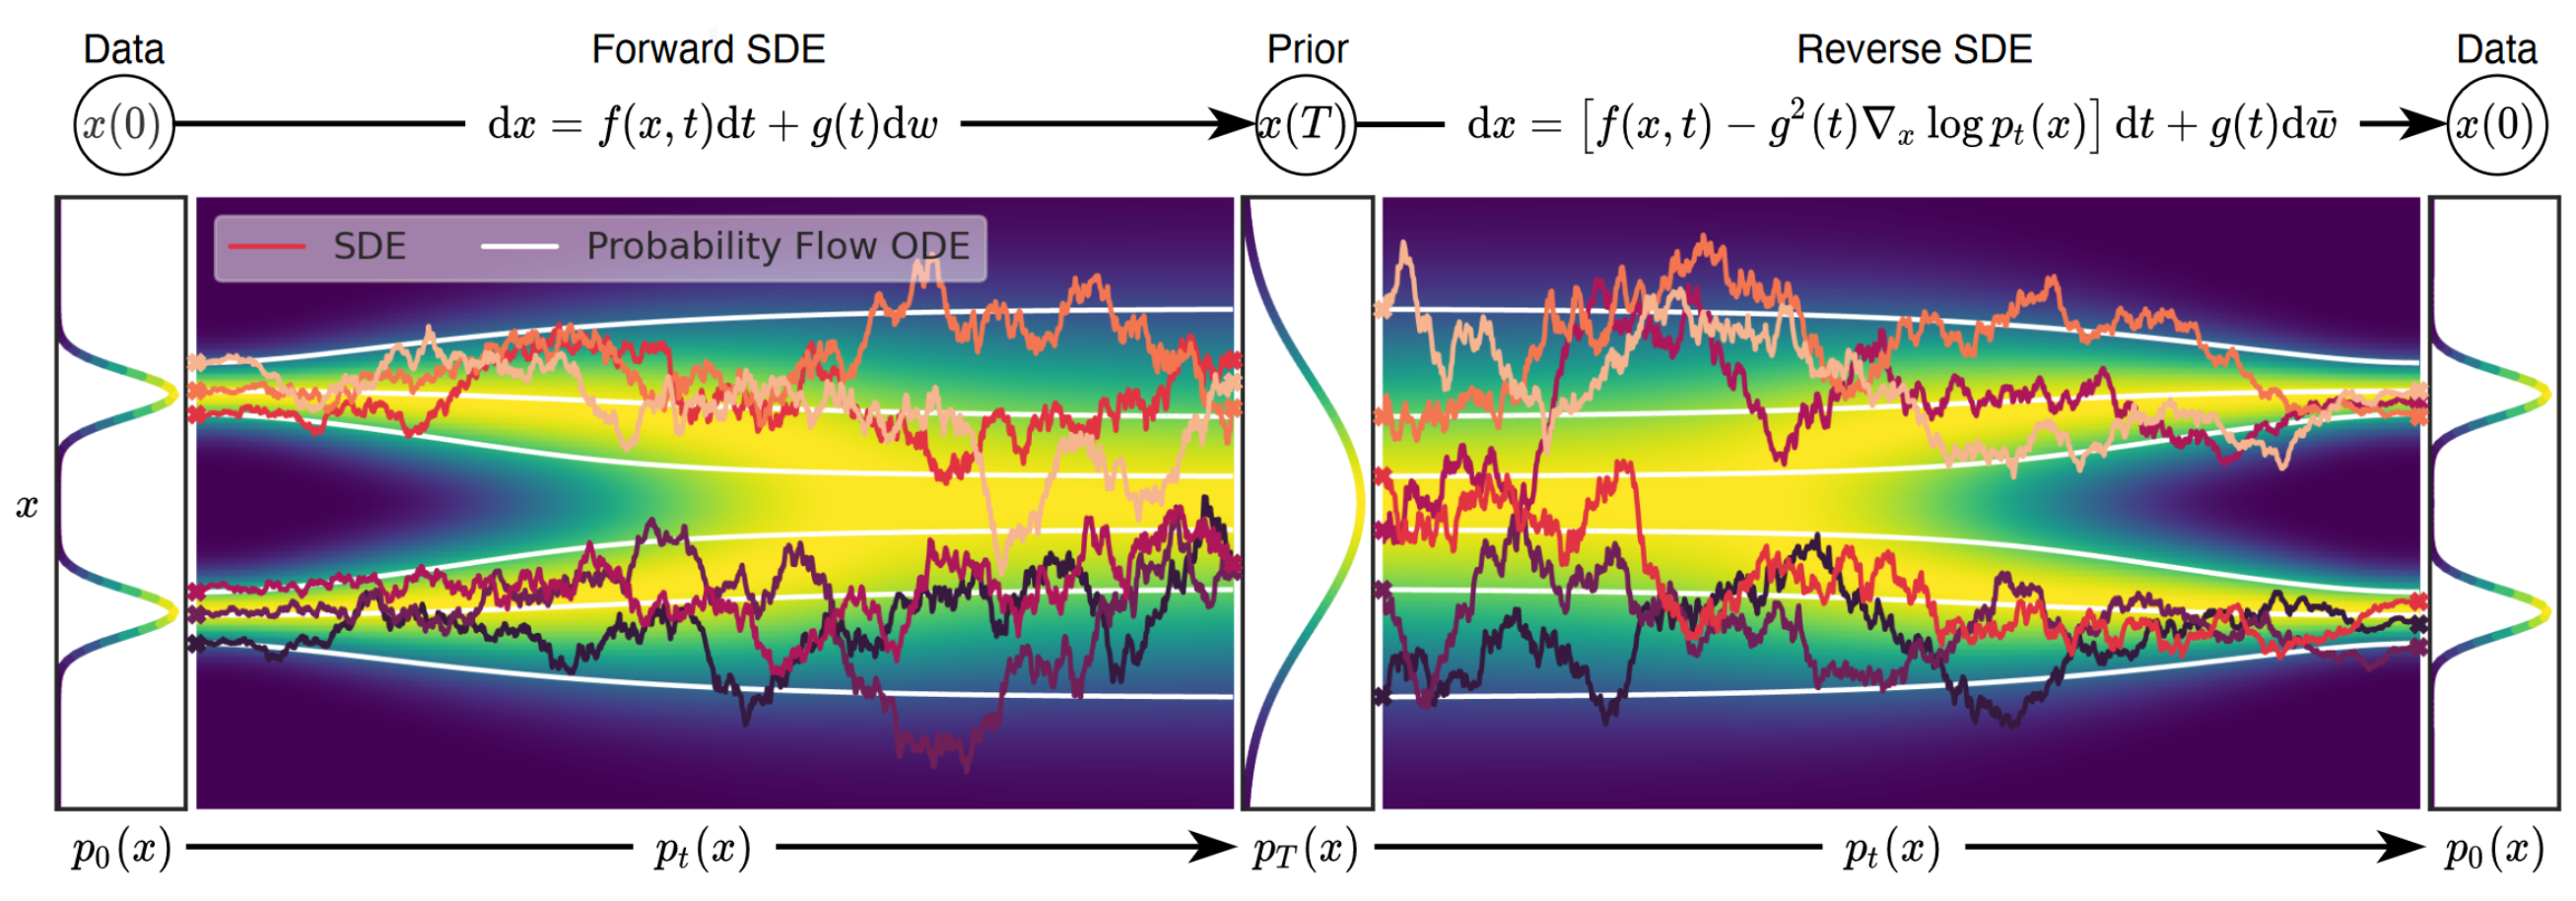
\includegraphics[width=1\columnwidth]{figures/basics/DiffusionModels_SDEs.png}
    \caption{This figure, adapted from Song et al.~\citep{song2020score}, illustrates the two-fold process in score-based generative modeling through SDEs. On the left, the Forward SDE represents the gradual transformation of data into noise, guided by the drift and diffusion coefficients. On the right, the Reverse SDE depicts the process of reconstituting original data from noise, leveraging the known score of each marginal distribution.}\label{fig:DM_SDEs}
\end{figure}

Training a model to accurately estimate the score functions at various noise levels is a fundamental aspect of this process. To achieve this, the model is trained through score matching \citep{hyvarinenScoreMatching}, which involves fine-tuning the model to closely approximate these score functions across a spectrum of noise levels \citep{song2020score}. The training objective is to minimize the discrepancy between the estimated and true scores over time, influenced by the noise. The score matching process matches the output of the score network with the true gradient of the log-likelihood over the course of the SDE, enabling the generation of realistic data samples from complex distributions.